\documentclass{article}
\usepackage{pgfplots}
\pgfplotsset{compat=1.18}

\begin{document}

\begin{figure}[h]
\centering
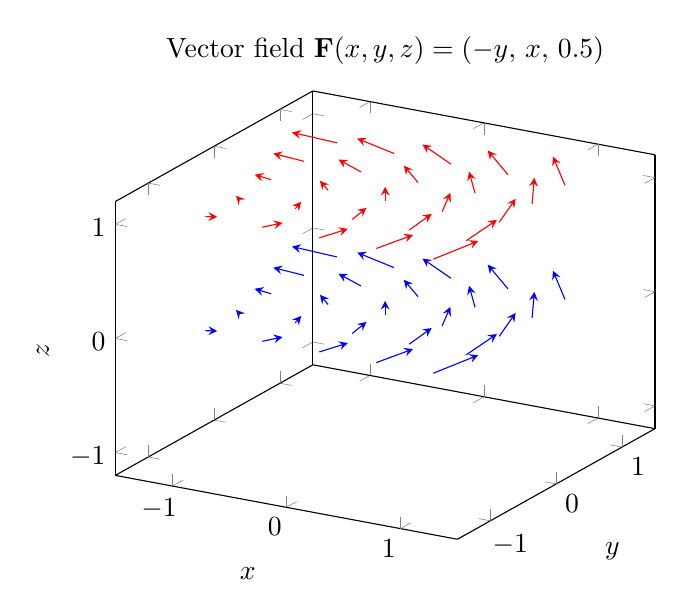
\begin{tikzpicture}
\begin{axis}[
    view={30}{25},
    xlabel=$x$, ylabel=$y$, zlabel=$z$,
    title={Vector field $\mathbf{F}(x,y,z) = (-y,\, x,\, 0.5)$},
    xmin=-1.5, xmax=1.5, ymin=-1.5, ymax=1.5, zmin=-1.2, zmax=1.2,
]
\addplot3[
    blue,
    -stealth,
    quiver={
        u={-y},
        v={x},
        w={0.5},
        scale arrows=0.25,
    },
    samples=5,
    domain=-1:1,
    domain y=-1:1,
] (x, y, {0});
\addplot3[
    red,
    -stealth,
    quiver={u={-y}, v={x}, w={0.5}, scale arrows=0.25},
    samples=5,
    domain=-1:1,
] (x, y, {1});
\end{axis}
\end{tikzpicture}
\caption{A rotational vector field with constant upward component.}
\end{figure}

\end{document}
